\documentclass{article}
\usepackage[utf8]{inputenc}
\usepackage[english]{babel}
\usepackage{amssymb}
\usepackage{amsmath}
\usepackage{graphicx}

\usepackage{geometry}
\geometry{left=2.5cm,right=2.5cm,top=2cm,bottom=2cm}

\setlength{\parskip}{0.5em}
\setlength{\parindent}{0em}
\renewcommand{\baselinestretch}{1.0}

\title{Assignment 1 Solutions}
\author{COL 352\\
    Introduction to Automata \& 
    Theory of Computation}
\date{}

\begin{document}
    \maketitle
    
    \section*{Problem 1} Consider the following two definitions of the strings of balanced parentheses:
    
    A. A string $w$ is balanced iff \\
    (i) $w$ has an equal number of "(" and ")"\\
    (ii) Any prefix of $w$ has at least as many "(" as ")"
    
    B. A string $w$ is balanced iff\\
    (i) $\epsilon $ is balanced.\\
    (ii) If $w$ is balanced, so is ($w$).\\
    (iii) If $w$ and $x$ are balanced then so is $w\textrm{·}x$\\
    (iv) Nothing else is balanced.
    
    Show that the above definitions A and B are equivalent.
    
    
    \textbf{Solution} : To show $A \iff B$,
    
    Case I : $A \Longrightarrow B$
    
    Proof : By induction on the length of the string $w$
    
    Basis : For $|w| = 0$, using B (i), $w$ is balanced
    
    Induction Hypothesis : Let string $w \in A$ then for all strings smaller than $w$, $A \Longrightarrow B$
    
    Induction Step:
    
    \quad Case(i) - $w$ does not have any prefix with equal number of "(" and ")" : 
    
    \qquad Then $w$ is of the form $( x )$ for some string $x$. 
    
    \qquad Since $x$ has equal number of "("and ")", and its prefixes have at least as many "(" as ")", so $x \in A$
    
    \qquad From IH,  $x \in B$
    
    \qquad From B (ii),  $w \in B$
    
    
    
    \quad Case(ii) - $w$ has a prefix $x$ with equal number of ”(” and ”)”
    
    \qquad Then $w$ is of the form $x.y$ for some shortest prefix $x$ and some $y \neq \epsilon$.
    
    \qquad Since $x$ and $w$ have equal number of ”(” and ”)”, hence $y$ will also have equal number of ”(” and ”)”.
    
    \qquad $y$ has at least as many ”(” as ”)” because, if some prefix of $y$ has less ”(” then $w$ will have less ”(”.
    
    \qquad But $w$ is balanced. So $x, y \in A$
    
    \qquad From IH, $x, y \in B$
    
    \qquad From B (iii), $w \in B$\\


Case II : $B \Longrightarrow A$
    
    Proof : By induction on the length of the string $w$
    
    Basis : For $|w| = 0$, using A (i) \& (ii), $w$ is balanced
    
    Induction Hypothesis : Let string $w \in B$ then for all strings smaller than $w$, $B \Longrightarrow A$
    
    Induction Step:
    
    \quad Case(i) - $w$ is balanced according to B (ii), i.e. $w = (x)$: 
    
    \qquad By IH, $x$ is balanced by $A$, i.e. $x$ has equal number o f ”(” and ”)” and so is ($x$)
    
    \qquad By IH, $x$ has atleast as many ”(” as ”)”, and so has ($x$)
    
    \qquad Thus, $w \in A$
    
    \quad Case(ii) - $w$ is balanced according to B (iii), i.e. $w = x.y$
    
    \qquad By IH, $x$ and $y$ are balanced by A, so $x$ and $y$ have equal 
    
    \qquad number of ”(” and ”)”, hence $x.y$ has equal number of ”(” and ”)”.
    
    \qquad If some prefix $z$ of $w$ has less ”(” than ”)”, then there are 2 cases :
    
    \quad \qquad (a) $z$ completely lies in $x$ - By IH, any prefix of $x$ cannot have fewer ”(” than ”)”, a contradiction.

    \quad \qquad (b) $z$ extends to $y$ -  Since $x$ has equal number of ”(” and ”)” and $z$ has fewer ”(” than ")", so prefix 
    
    \quad \qquad of $y$ has fewer ”(”. But by IH, prefix of $y$ cannot have less ”(” and ”)”, a contradiction.
    
    \qquad Thus, $w \in A$
    
    
    \section*{Problem 2} Show that the Principle of Mathematical Induction and the Principle of Complete induction are equivalent.
Hint: Express them rigorously as sentences in first order logic.

    \textbf{Solution} : 
    Let $A$ denote Principle of Mathematical Induction and $B$ denote Principle of Complete Induction. To show $A \iff B$,
    
    Case I : $A \Longrightarrow B$
    
    Proof : Let $Q(K) = P(1) \& P(2) \& P(3) ... \& P(k)$ , be the preposition that denotes whether $P(i) = true \forall i \leq K$
    
    \quad $Q(K) \Longrightarrow Q(K + 1)$ from premise (Invoking Math Induction on $Q(k)$ ---(1)
    
    \quad $Q(K) \Longrightarrow P(K)$ from definition of $Q(K)$ ---(2)
    
    \quad Invoking math induction on $P(K),  P(K) \Longrightarrow P(K + 1)$ ---(3)
    
    \quad Using (2) and (3) and applying transitive law we get, $Q(K) \Longrightarrow P(K + 1)$
    
    Case II : $B \Longrightarrow A$
    
    Proof : From the premise, $((P(1) \& P(2) \& P(3) ... \& P(k)) \Longrightarrow P(k + 1)$
    
    \quad $\Longrightarrow (Q(k - 1) \& P(k)) \Longrightarrow P(k + 1)$
    
    \quad $\Longrightarrow \neg (Q(k - 1) \& P(k)) \lor P(k+1)$

    \quad $\Longrightarrow \neg Q(k - 1) \lor \neg P(k) \lor P(k+1)$

    \quad $\Longrightarrow \neg Q(k - 1) \lor (P(k) \Longrightarrow P(k + 1))$
    
    \quad So, to prove mathematical induction holds we prove that proposition $Q(k - 1)$ is true.
    
    \quad Let us assume on the contrary that $Q(k - 1)$ is false
    
    \quad $\Longrightarrow \exists i, P(i) = false, i \leq (k - 1)$
    
    \quad $\Longrightarrow \exists i', P(i') = false, i' \leq i$
    
    \quad The sequence of $i$’s forms a strictly decreasing sequence and will terminate at $i = 1$, i.e. $P(1) = false$.

    \quad This contradicts the hypothesis of complete induction, hence $P(K) \Longrightarrow P(K + 1)$
    
    \quad Hence mathematical induction holds.
    
    \section*{Problem 3} Show two distinct bijective mappings between integers and rationals.
    
    \textbf{Solution} : 
    
\quad \textbf{Bijection 1} - For $i \in \mathbb{N}$, define $T(i)=\begin{cases}
                \frac{-i}{2}, & \hbox{if i is even;} \\
                \frac{i+1}{2}, & \hbox{if i is odd.}
            \end{cases}$
     Then $T$ is a bijection from $\mathbb{N}$ to $\mathbb{Z}\setminus\{0\}$

    \quad If $n = \prod_{k}p_k^{n_k}$
    
    \quad define $f: \mathbb{N}\rightarrow \mathbb{Q^+}$ by $f(n)=\prod_{k}p_k^{T(n_k)}$
    
    \quad Claim : f is a bijection
    
    \quad I. f is one-one
    
    \qquad If $f(m) = f(n)$, we have two rational numbers which are equal and thus have the same fractional representation $\frac{p}{q}$ with $p,q \in \mathbb{N}$. Writing the fraction as a prime factorization, we get a product like $\prod_{k}p_k^{y_k}$, where $y_k$ are positive or negative integers. We map the $y_k$ to the inverse of the $T$ transformation to get the $n_k$ and thus the $n$. Hence function $f$ is one-one.
    
    \quad II. f is onto
    
    \qquad Let $\frac{p}{q}=\prod_{k}p_k^{y_k}$, where $y_k$ are positive or negative integers, be any rational number. 
    
    \qquad Choose $n_k = T^{-1}(y_k)$ 
    
    \qquad If $n=\prod_{k}p_k^{n_k}$, then we have $f(n)=\prod_{k}p_k^{T(n_k)}=\prod_{k}p_k^{y_k}=\frac{p}{q}$ 
    
    \qquad Therefore there exists a natural number $n$ for each given rational number $\frac{p}{q}$ such that $f(n)=\frac{p}{q}$. 
    
    \qquad Hence $f: \mathbb{N}\rightarrow \mathbb{Q^+}$ given by $f(n)=\prod_{k}p_k^{T(n_k)}$ is a bijection.
    
    
    \qquad Define $g: \mathbb{Z} \rightarrow \mathbb{Q}$ such that
    
    \qquad $g(n)=
    \begin{cases}
        f(n), & \hbox{if $n>0$;} \\
        f(-n), & \hbox{if $n<0$;} \\
        0, & \hbox{if $n=0$.}
    \end{cases}$
    
    \qquad Since $f$ is bijection so $g$ is also a bijection. 
                
    \quad \textbf{Bijection 2} - The set $\mathbb{Q^+}$ of positive rational numbers can be written as follows

    \begin{center}
    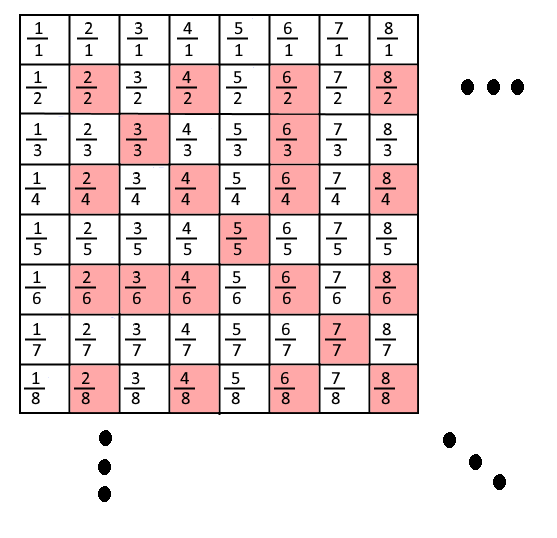
\includegraphics[width=3.5 in]{Images/q4-1.png}
    \end{center}
    
    \quad We map natural numbers diagonally on this array as follows
    
    \begin{center}
    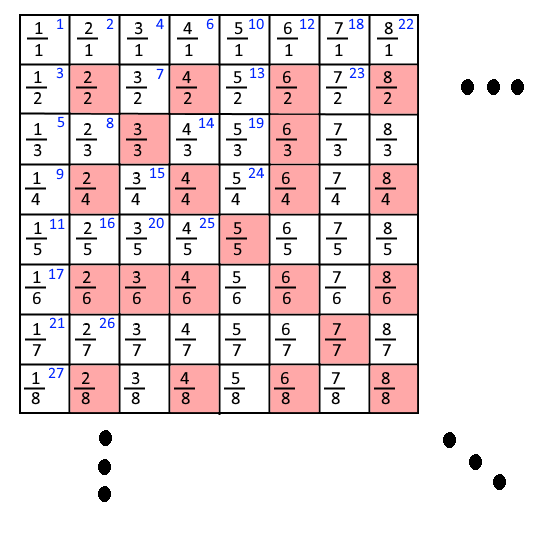
\includegraphics[width=3.5 in]{Images/q4-2.png}
    \end{center}
    
    \quad Numbers in blue are natural numbers. 
    
    \quad Let $f$ denote this bijection of natural numbers to set of positive rational numbers.
    
    \quad Note that this array contains each natural number exactly once and each positive rational number is image of some natural number so the array given above represents a bijection from natural numbers to positive rational numbers. 
    
    \quad Define $g: \mathbb{Z}\rightarrow \mathbb{Q}$ such that $g(n)= \begin{cases}
        f(n), & \hbox{if $n>0$;} \\
        f(-n), & \hbox{if $n<0$;} \\
        0, & \hbox{if $n=0$.}
    \end{cases}$

    \quad Since $f$ is bijection, $g$ is also a bijection.

    \section*{Problem 4}  A relation $ \leq_{\#}$ is defined as follows - If $A, B$ are sets, then $A \leq_{\#} B$ iff there exists a 1-1 mapping $f : A \rightarrow B$ and an onto mapping $g : B \rightarrow A$. $If f : A \rightarrow B$ is a bijection then, $A\leq_{\#} B$.
    
What can you say about the pairs of sets

(i) integers and rationals (ii) Reals in [0, 1] and reals in $(10, 100)$ (open interval)

The Bernstein-Schroeder theorem says that If $A \leq_{\#} B$ and $B \leq_{\#} A$ then $A =_{\#} B$.
    
\textbf{Solution} :

    (i) Using the bijection found between Rationals and Integers in Problem 4, by the second clause $\mathbb{Z} =_{\#} \mathbb{R}$
    
    (ii) Let $f(x): [0,1] \to (10, 100)$  be defined as : $f(x) = 
        \begin{cases}
               x+11 & \quad if x \in (0, 1)\\
               12 & \quad if x = 0\\
               13 & \quad if x = 1 \\
            \end{cases}$
            
    \quad For a one-one function, if $f(x) = f(y)$ then $x = y$
    
    \quad Case 1 : $x=0, y=1$
    
    \quad $f(x)=12, f(y)=13, ~ f(x) \neq f(y)$
    
    \quad Case 2: $x=0, y \in (0, 1)$
    
    \quad $f(x)=12, f(y) \in (11, 12), ~f(x) \cap f(y) = \phi $
        
    \quad Case 3: $x=1, y \in (0, 1)$
    
    \quad $f(x)=13, f(y) \in (11, 12), ~f(x) \cap f(y) = \phi$
        
    \quad Therefore f(x) is a one-one function 
    
    \quad Let $g(x): (10, 100) \to [0, 1]$  be defined as:
    $g(x) = 
         \begin{cases}
           x-20 &\quad if x \in [20, 30] \\
           0 &\quad otherwise
         \end{cases}$
    
    \quad Let $y=x-20$ for $x \in[20, 30] \implies x=y+20, ~\forall y \in [0, 1] $
    
    \quad $\implies x \in [0+20, 0+30] \implies x \in [20, 30]$
    
    \quad Thus $g(x)$ is onto 
    
    \quad Since $f(x): [0,1] \to (10, 100)$ is one-one and $g(x): (10, 100) \to [0, 1]$ is onto, therefore $[0, 1] <_{\#} (10, 100)$ 
    
    
    \quad Let $f(x): (10, 100) \to [0, 1]$  be defined as:
    $f(x) =  \frac{x-10}{90}$
    
    \quad Let $ f(x_{1})=f(x_{2}) $
    
    \quad $\implies \frac{x_{1}-10}{90}=\frac{x_{2}-10}{90} $ 
    
    \quad $\implies x_{1}=x_{2}$ 
    
    \quad Therefore $f(x)$ is one-one 
    
    \quad Let $g(x): [0,1] \to (10, 100)$  be defined as:
    $g(x) = 
         \begin{cases}
           90x+10 \quad if x \in (0,1) \\
           20  \quad if x \in \{0, 1\} 
         \end{cases}$
        
    \quad Let $y=90x+10$ for $x \in (0,1)$
    
    \quad $\implies x=\frac{y-10}{90}, ~ \forall
     y \in (10, 100), x \in (\frac{10-10}{90}, \frac{100-10}{90}) $
     
    \quad $\implies x \in (0, 1) $
    \quad Thus, $g(x)$ is onto 
    
    \quad Since $f(x): (10, 100) \to [0, 1]$ is one-one and $g(x): [0,1] \to (10, 100)$ is onto, therefore $(10, 100) <_{\#} [0, 1]$ 
    
    
    \quad Thus by equation 4 and 7 and Bernstein-Schroeder theorem, $[0, 1] =_{\#} (10, 100) $
    
    
\end{document}
